\chapter{The Spectral Algorithms}\label{chapter:2}
In this chapter, we focus on the the case SNR $>1.$ Specifically, we revisit the standard spectral algorithms and non-backtracking matrix based spectral algorithm which is used to prove theorem $\ref{thm:1.1.1}.$\\
Spectral methods typically refer to the approach of partitioning the nodes into groups by using the  spectral properties of the graph matrices \cite{dallamico:tel-03454227}. The eigenvalue spectrum of various graph matrices, such as the adjacency matrix, the Laplacian, and the non-backtracking matrix, usually consists of a compact bulk of closely spaced eigenvalues, along with some outlying eigenvalues separated from the bulk. The eigenvectors corresponding to these outliers often  provide insights into the large-scale structure of the network, including its community structure \cite{userguide}. Therefore, it enables us to detect the communities in  a graph by utilising the the eigenvectors corresponding to these outlying eigenvalues.
\section{Standard Spectral Algorithm}
The standard spectral algorithm refer to spectral algorithms based on adjacency or Laplacian matrix. \\
It has been demonstrated that for a given graph with community structure and SNR $>1$, the eigenvector corresponding to the second largest eigenvalue of its adjacency matrix is correlated with the true community structure when the graph is sufficient dense \cite{standard_spec_in_dense}. Therefore, the spectral algorithm based on the adjacency matrix can compute community labels by simply labelling vertices according to the sign of the second eigenvector for the case of two communities ($k=2$). This approach can be generalised to the case of more than two communities ($k>2$) by applying heuristic techniques such as the k-means algorithm.\\
However, this correlation diminishes in sparse graphs (i.e., $c$ is constant while $n\to\infty$), as detailed in \cite{the_non-backtracking}. In sparse graphs, eigenvectors corresponding to eigenvalues outside the bulk may correlate with high-degree vertices rather than the community structure. Similarly, community-related eigenvalue could be merged into the bulk, the community-correlated eigenvector with uninformative eigenvectors. As a consequence, identifying the community-correlated eigenvector becomes challenging or even impossible. The same issue arises when using the Laplacian matrix.\\
One potential remedy is to remove the high-degree vertices, but this approach discards a significant amount of information and can cause the graph to disintegrate into disconnected components \cite{TheConjecture}. Therefore, an alternative method is required to mitigate the influence of high-degree vertices while preserving the community structure information.

\section{Spectral Algorithm based on Non-backtracking Matrix}\label{sec: Spectral Algorithm based on Non-backtracking Matrix}
The non-backtracking matrix, as defined in definition \ref{def: non_backtracking}, is introduced to address this issue. Due to its non-backtracking nature, i.e., a vertex cannot be revisited within two steps, the non-backtracking matrix is less sensitive to high-degree vertices compared to the adjacency or Laplacian matrices.\\
Let $\mu_i$ denote the \textit{i-th} largest eigenvalue of the non-backtracking matrix, $\lambda_i$ denote its corresponding eigenvector.
it was shown in \cite{the_non-backtracking} that the non-backtracking matrix has the following spectrum properties:
\begin{theorem}\label{thm: 2.2.1}
    Let $G$ be a realisation of $SSBM(n, 2, p_{in}, p_{out}).$ If $(c_{in}-c_{out})/2>\sqrt{c},$ then, with high probability, the two largest eigenvalues of $\mathbf{B}$ are real and satisfy
    \begin{itemize}
     \vspace{-5mm}
        \item $\mu_1\to c$
        \vspace{-3mm}
        \item $\mu_2\to(c_{in}-c_{out})/2$
        \vspace{-3mm}
        \item $|\mu_{i_{>2}}|\leq\sqrt{c},$ i.e. the radius of the bulk of $\mathbf{B}$'s is confined in $\sqrt{c}$
    \end{itemize}
\end{theorem}
\begin{remark}
    the constraint $(c_{in}-c_{out})/2>\sqrt{c}$ is equivalent to SNR $>1.$
\end{remark}
Krzakala et al. \cite{the_non-backtracking} point out that the eigenvector $\lambda_2$ is strongly correlated with the true community structure. Moreover, according to Theorem \ref{thm: 2.2.1}, $\mu_2$, the second largest eigenvalue of the non-backtracking matrix $\mathbf{B}$, is well-separated from the bulk of $\mathbf{B}$'s spectrum for SNR > 1, regardless of whether the graph is sparse or dense. Figure \ref{fig: spectrum} illustrates an example of the spectrum of $\mathbf{B}$, showcasing this separation.
\begin{figure}
    \centering
    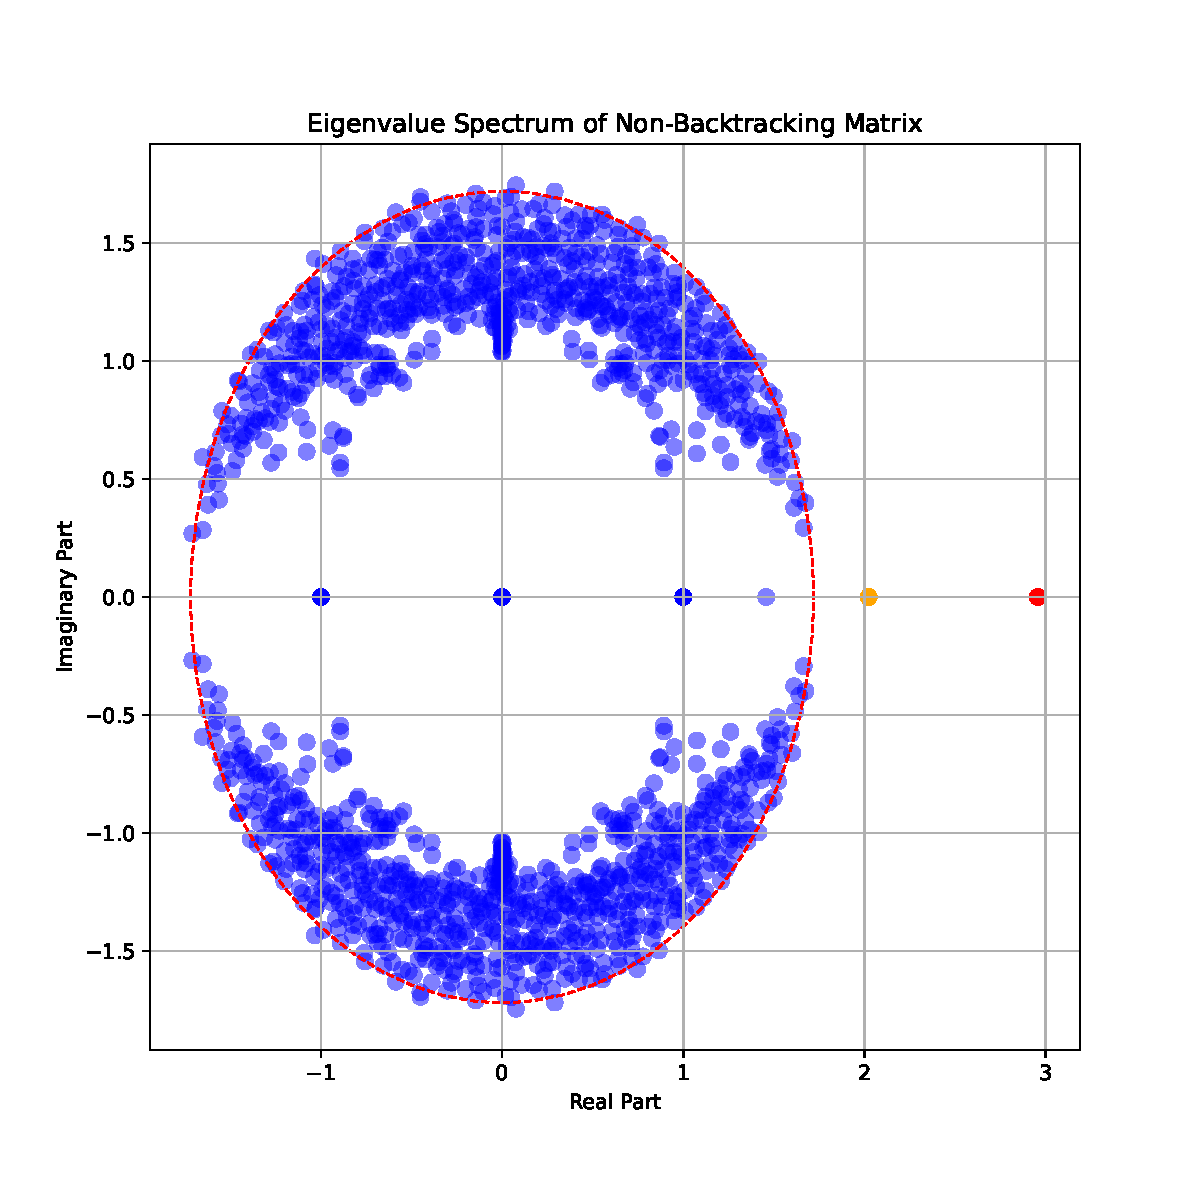
\includegraphics[width=1\linewidth]{Figures/spectrum_plot.pdf}
    \caption[Spectrum distribution of non-backtracking matrix]{The spectrum of the non-backtracking matrix of a graph drawn from $SSBM$ with parameters $n=10^3,~k=2,~c_{in}=5,~c_{out}=1.$ In this scenario, SNR $=4/3$ and we can observe that $\mu_2$ is well-separated from bulk of spectrum. Moreover, $\mu_1\to3=(c_{in}+c_{out})/2=c$, $\mu_2\to2=(c_{in}-c{out})/2$ and the radius of the bulk is $\sqrt{c}=\sqrt{3},$ These observations are in alignment with Theorem $\ref{thm: 2.2.1}.$}
    \label{fig: spectrum}
\end{figure}

Therefore, the spectral algorithm based on non-backtracking matrix validates Theorem \ref{thm:1.1.1}. The algorithmic procedure of this spectral algorithm is summarized in Algorithm \ref{algo1}.

\begin{algorithm}[H]\label{algo1}
\SetAlgoLined       % This enables vertical lines to indicate block levels
\SetKwInput{KwInput}{Input}                % Set the Input
\SetKwInput{KwOutput}{Output}              % Set the Output
\LinesNumbered
\KwInput{Graph $G=(V, E)$ drawn from $SSBM(n, 2, p_{in}, p_{out})$}
\KwOutput{Computed communities assignment $\sigma'$}
\Begin{
Convert $G$ into a directed graph;\\
$\mathbf{B}\leftarrow$ non-backtracking matrix of $G$;\\
$\xi\leftarrow$ eigenvector corresponding to the second largest eigenvalue;\\
\For{$v\in V$}{
  \If{$\sum_{\{(u,v)\in E:~\text{head is}~v\}}\xi_{(u, v)}>0$}{$\sigma_v'\leftarrow$ Community A;}
  \Else{$\sigma_v'\leftarrow$ Community B;}
}
\Return{$\sigma'$}
}
\BlankLine
\caption{Spectral Algorithm base on Non-Backtracking Matrix}
\end{algorithm}
\vspace{6mm}
Figure \ref{fig:spec_algo} presents the experimental results of Algorithm \ref{algo1}. These results are consistent with those reported in \cite{the_non-backtracking}.
\begin{figure}[H]
    \centering
    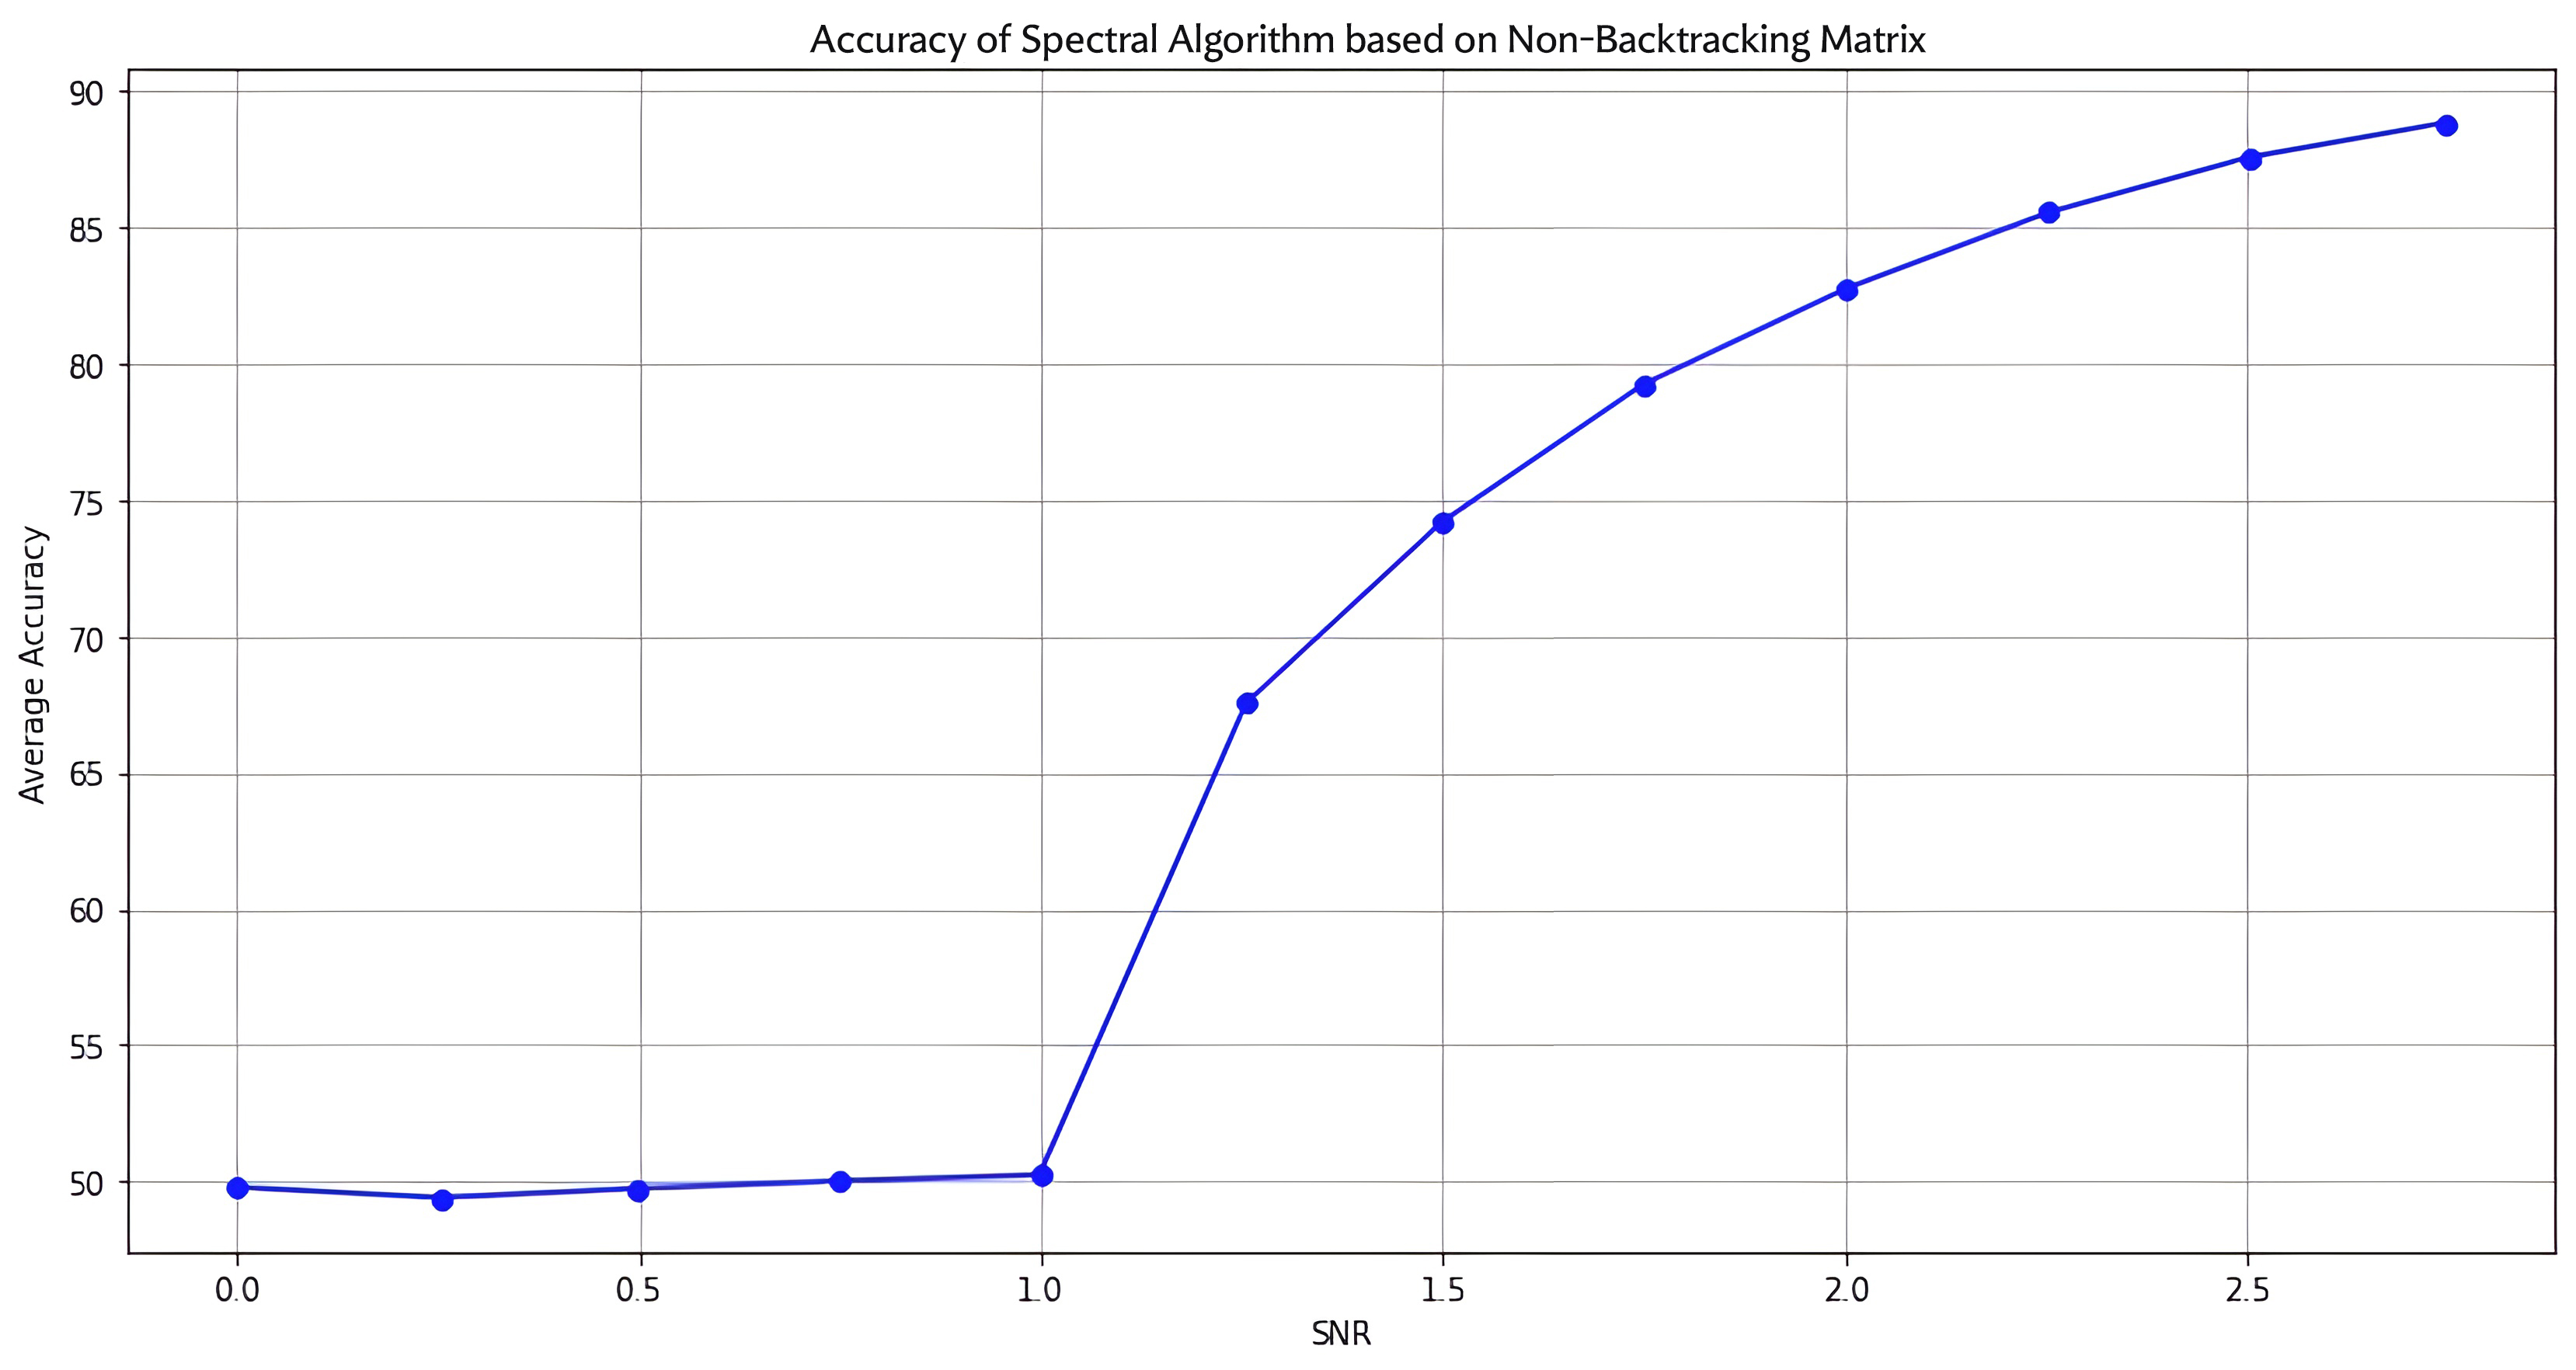
\includegraphics[width=1\linewidth]{Figures/spec_algo.jpg}
    \caption[Accuracy of the spectral algorithm based on non-backtracking matrix]{The accuracy of spectral algorithm based on non-backtracking matrix across different SNR values. The experiment is averaged over 10 instances with $n=10^4$ and $c=3.$}
    \label{fig:spec_algo}
\end{figure}
From Figure \ref{fig:spec_algo}, we observe that when SNR > 1, the spectral algorithm based on the non-backtracking matrix noticeably outperforms random guessing, which has an expected accuracy of 50\% across all SNR values.
